\chapter{Estudio teórico. Propuestas en Positional Encoding}

En el capítulo anterior, presentamos los principales modelos de aprendizaje para series temporales, y así analizar las soluciones propuestas por cada uno. Al hacerlo, pudimos identificar un problema clave: la codificación posicional no recibe la atención necesaria, y en la mayoría de casos se usa la formulación original, con adaptaciones mínimas, o bien, es suprimido a favor de otras alternativas incorporadas en la propia arquitectura.\\

En este capítulo, teniendo presente los tipos anteriormente descritos de codificaciones (fijo, aprendible, adición de variables temporales, transformaciones), retomaremos esa clasificación para profundizar en las propuestas más recientes orientadas específicamente a series temporales, analizando su motivación, diseño y posibles ventajas frente a las formulaciones clásicas.\\

Partiremos del esquema tradicional de codificación posicional heredado del Transformer original y examinaremos cómo distintos trabajos recientes han intentado superar sus limitaciones mediante adaptaciones de carácter local o dependientes del contenido. Nuestro objetivo será identificar las ventajas concretas que aporta cada enfoque, extraer de ellos la inspiración necesaria y, a partir de ahí, diseñar nuevos experimentos de codificación posicional que integren ideas capaces de mejorar el rendimiento del modelo.

\section{Análisis de propuestas existentes}

Durante el análisis de los modelos más destacados del estado del arte, hemos podido ver en uso, principalmente, el mecanismo tradicional de atención basado en senos y cosenos, así como el basado en las transformadas de Fourier y Wavelet, en el caso de FEDformer. Sin embargo, dejando al margen estos enfoques, no hemos apreciado ninguna otra alternativa intuitiva que trate de mejorar el positional encoding más allá, ya que en otros casos, directamente se opta por su supresión o compensación por otro mecanismo.\\

Para poder profundizar más en este aspecto, podemos adentrarnos en surveys como el publicado por \textit{Habib Irani y Vangelis Metsis}~\cite{irani2025positionalencodingtransformerbasedtime}, donde se recogen multitud de variantes de encoding, aplicados a series temporales. Tomando como referencia la clasificación propuesta (ver figura \ref{encodings}), a continuación agruparemos las codificaciones posicionales en dos grandes categorías. Por un lado, aquellas que se incorporan sumándose directamente al embedding de entrada, conocidas como métodos absolutos de codificación posicional (APE); por otro, las que actúan modificando el propio cálculo de la atención, y que por ello se denominan métodos relativos de codificación posicional (RPE).


\begin{figure}[!ht]
	\centering
	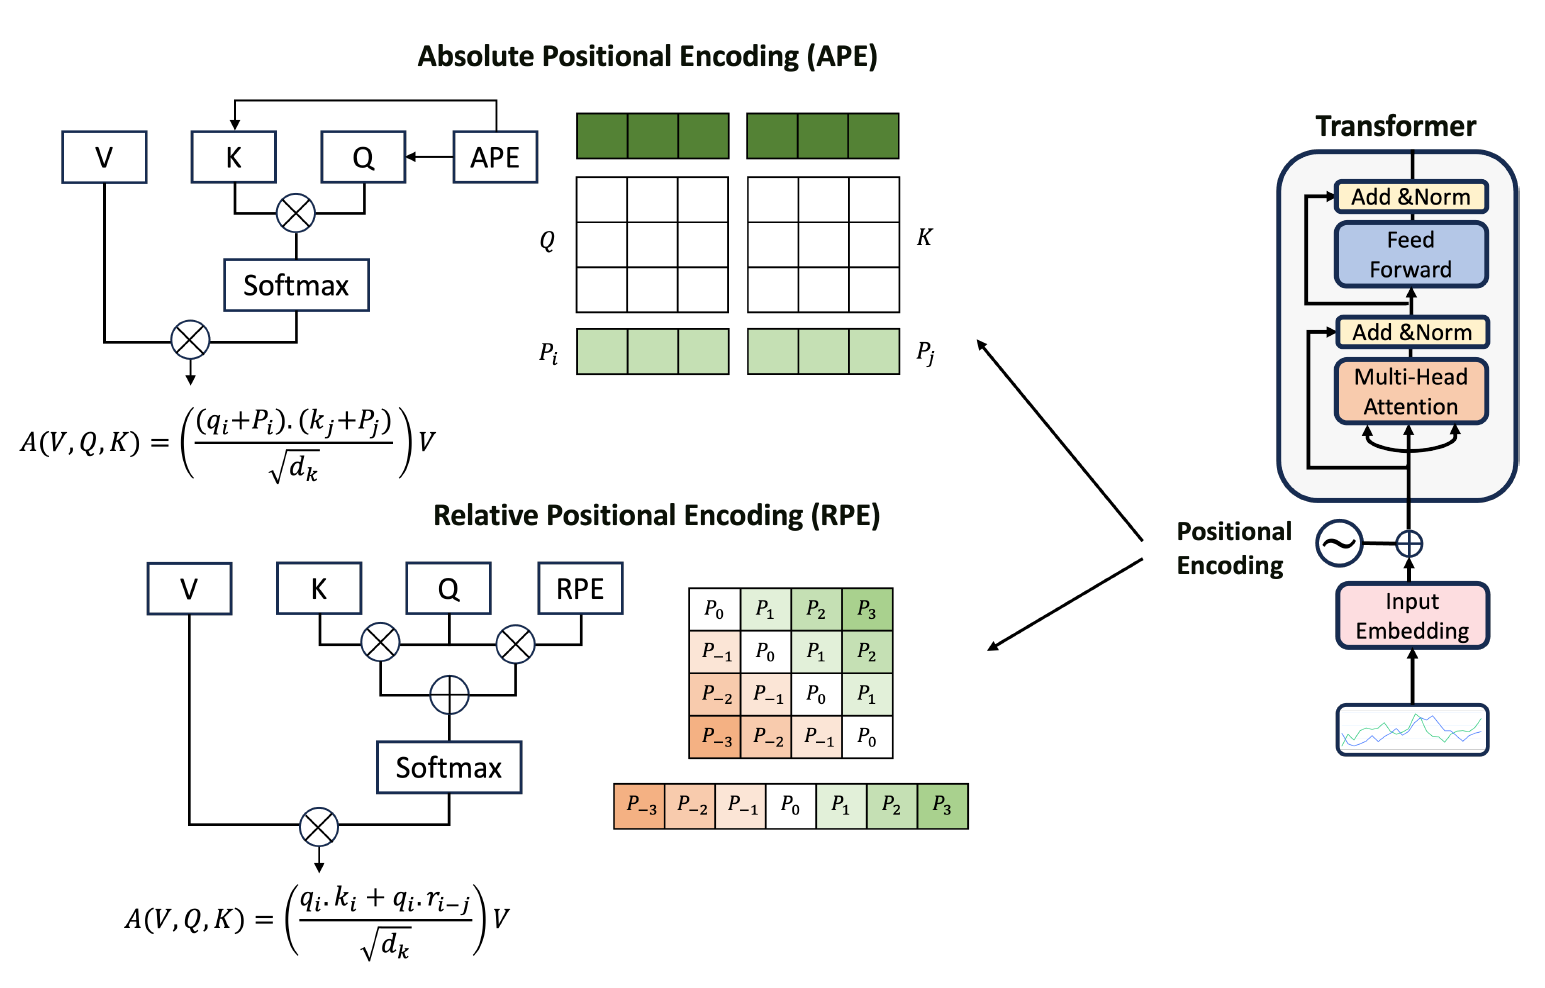
\includegraphics[scale=0.275]{img/encodings.png}
	\caption{Encodings: clasificación de métodos y funcionamiento \cite{irani2025positionalencodingtransformerbasedtime}}
	\label{encodings}
\end{figure}

\subsection{Métodos aditivos}

Comenzaremos el análisis por el positional encoding aditivo. Esta vertiente toma como referencia el mecanismo de adición de información empleado por el enfoque sinusoidal original, ya que todas estas codificaciones se añaden al embedding mediante suma, de forma que no es necesario realizar modificaciones adicionales a la arquitectura neural que los procesará, y facilita el uso de modelos preentrenados con el fin de ahorrar recursos de cómputo.\\

En mayor detalle, estos métodos construyen un vector posicional $(P \in \mathbb{R}^{L \times d})$ y lo se suma directamente a los embeddings de entrada (X), obteniendo:

$$ X' = X + P $$

donde (L) es la longitud de la secuencia y (d) la dimensión del embedding.\\

Suponen una ventaja desde el punto de vista de la usabilidad, ya que modificar excesivamente los mecanismos de atención puede dificultar su comprensión y provocar efectos adversos indeseados si no se realiza con el rigor necesario. A continuación, destacaremos algunos de los mecanismos existentes con estas características, y analizaremos la utilidad ofrecida por cada uno.

\subsubsection{Sinusoidal Positional Encoding (PE)}

Se trata del encoding original propuesto originalmente por Vaswani et al. (2017)~\cite{vaswani2023attentionneed}, a modo de recordatorio. Como ya vimos, utiliza funciones sinusoidales para representar la posición:

$$
PE_{(pos, 2i)} = \sin\left(\frac{pos}{10000^{\frac{2i}{d}}}\right)
$$

$$
PE_{(pos, 2i+1)} = \cos\left(\frac{pos}{10000^{\frac{2i}{d}}}\right)
$$

Donde cada variable indica:

\begin{itemize}
	\item \textbf{pos}: índice temporal (posición).
	\item \textbf{i}: dimensión del componente del embedding.
	\item \textbf{d}: dimensión total del embedding.
\end{itemize}

Basándonos simplemente en su formulación, fuimos capaces de distinguir ya sus ventajas y desventajas; como ventaja, podemos ver que se trata de una codificación no entrenable, por lo que para unas mismas dimensiones de entrada de datos, el resultado será siempre el mismo, y sus valores no se deben entrenar época a época de manera independiente. Esto lo hace más sencillo de usar, y más eficiente al no requerir parámetros adicionales. Sin embargo, como principal desventaja, estimamos que no permite modelar con suficiente adaptabilidad los períodos no estacionales de datos o con mayor número de irregularidades y valores anómalos.\\

Su forma sencilla de acoplar al conjunto de datos de entrada nos sirve de inspiración para la creación de nuevas variantes que traten de incorporar más contexto semántico de los datos.

\subsubsection{Time Absolute Positional Encoding (tAPE)}

tAPE propone una solución que, aunque sigue perteneciendo a la familia de codificaciones fijas, incorpora información estructural propia de la secuencia de entrada, en particular su longitud real $L$. La idea central es ajustar la escala de las frecuencias empleadas en la codificación sinusoidal en función de esa longitud, de forma que la representación posicional conserve una propiedad conocida como \textit{distance-awareness}.\\

Por \textit{distance-awareness} entendemos la capacidad de la codificación para reflejar, de manera coherente y diferenciada, la distancia relativa entre posiciones, y así complementar a la información global. En una codificación con buena distance-awareness, dos posiciones cercanas deben tener representaciones más similares entre sí que respecto a posiciones muy alejadas, y esta relación se mantiene de forma proporcional a lo largo de toda la secuencia. Es algo que no logramos cosneguir en codificaciones sinusoidales estándar, sobre todo cuando la dimensión del embedding es baja, ya que las frecuencias asignadas no siempre proporcionan suficiente resolución para representar distancias cortas.\\

Para mitigar este problema, tAPE redefine las frecuencias como:

\begin{equation}
	\centering
	\omega^{new}_k = k \cdot \frac{d_{model}}{L}
\end{equation}

Adaptando así su espectro al tamaño real de la secuencia y adecuándose incluso a casos de entrada de corta longitud. Esta nueva frecuencia simplemente se incorpora como parámetro a la codificación sinusoidal estándar:

\begin{equation}
	\begin{aligned}
		\text{PE}_{(pos,2i)} &= \sin\!\left( pos \cdot \omega^{new}_i \right) \\
		\text{PE}_{(pos,2i+1)} &= \cos\!\left( pos \cdot \omega^{new}_i \right)
	\end{aligned}
\end{equation}


Donde:

\begin{itemize}
	\item \textit{d} representa la dimensión del embedding utilizada por el modelo Transformer; este valor determina el número de componentes de la codificación posicional y, por tanto, el rango de frecuencias disponibles para representar las posiciones.
	\item \textit{L} corresponde a la longitud real de la secuencia.
	\item \textit{k} es el índice de la dimensión o de la frecuencia dentro del embedding; al recorrer k desde valores bajos a altos, obtenemos frecuencias cada vez más elevadas en las funciones seno y coseno, lo que permite representar tanto variaciones lentas (baja frecuencia) como rápidas (alta frecuencia) a lo largo de la secuencia.
\end{itemize} 

La principal virtud de tAPE es su capacidad para mantener la distance-awareness incluso en contextos con embeddings de baja dimensión, algo que no siempre se logra con la codificación sinusoidal estándar. Al incorporar la longitud real \textit{L} en el cálculo de las frecuencias, se evita que la escala sea excesivamente grande o pequeña para la secuencia procesada, lo que redunda en una representación posicional más ajustada y fiel a las distancias relativas. Esta adaptación es especialmente útil en series temporales de corta o media duración, donde las relaciones locales y su correcta discriminación son fundamentales.\\

Sin embargo, sigue teniendo limitaciones evidentes. Para empezar, su dependencia explícita de \textit{L} puede suponer un problema si, durante la inferencia, trabajamos con secuencias de longitud muy distinta a la usada en el entrenamiento, aunque normalmente, se deberían seguir distribuciones similares. Además, tAPE es un método de codificación fijo y no incorpora parámetros aprendibles, lo que si bien simplifica su uso y evita sobreajuste, también le impide adaptarse dinámicamente a patrones posicionales más complejos o irregulares presentes en diferentes dominios o conjuntos de datos.

\subsubsection{Learnable Positional Encoding (LPE)}

En el método sinusoidal tradicional, la codificación posicional se realizaba de forma fija e invariante, dependiendo únicamente de las dimensiones de los datos de entrada. Sin embargo, esto no favorece a la localización de estructuras y detalles propios de los datos de entrada, por lo que surge así el encoding posicional aprendible. Su filosofía se basa en dejar que el modelo sea quien entrene los valores de la codificación posicional a la vez que el resto de la arquitectura se refina:

$$
PE_{\text{learnable}}(pos) = W_{pos}, \quad W_{pos} \in \mathbb{R}^d
$$

Esta codificación aprendida se incorpora al embedding de entrada de manera aditiva como hasta ahora:


$$
X' = X + PE_{\text{learnable}}[pos]
$$

La principal fortaleza de este método reside en su capacidad de adaptación. A diferencia de métodos como el PE sinusoidal o tAPE, que imponen un patrón posicional fijo, LPE permite que el modelo aprenda directamente, a partir de los datos, la representación posicional que mejor captura las relaciones temporales y estructurales relevantes para la tarea. Esta flexibilidad puede traducirse en una mayor precisión, especialmente en dominios donde las dependencias posicionales no siguen un patrón excesivamente regular, o cuando la información contextual es altamente específica del conjunto de datos y es compleja de detectar de manera intuitiva.\\

No obstante, esta flexibilidad tiene un precio. Al añadir un vector de parámetros por cada posición, el tamaño del modelo crece linealmente dependiendo del parámetro de longitud \textit{L}, lo que incrementa tanto el coste de almacenamiento como el de entrenamiento. Además, la codificación aprendida queda estrechamente ligada al conjunto de datos utilizado para ajustarla; esto implica que, ante un cambio de dominio o de distribución de las secuencias, incluso si la longitud se mantiene, es necesario volver a entrenar los embeddings posicionales desde cero para preservar su utilidad. En contraste con tAPE, que conserva su aplicabilidad en distintos contextos gracias a su formulación fija, LPE sacrifica generalidad en favor de especialización.


\subsection{Métodos que manipulan la atención}

Hasta ahora, hemos explorado tres métodos de codificación posicional que comparten un rasgo común: todos operan mediante una simple suma dentro del embedding de entrada. Sin embargo, existe otra vía para mejorar el desempeño de los modelos Transformer que va más allá de la manipulación directa del embedding: intervenir directamente en el mecanismo de atención.\\

Hasta el momento, las modificaciones de atención que hemos visto se basaban principalmente en técnicas de muestreo para reducir el tamaño del producto, seleccionando un subconjunto de productos en lugar de trabajar con la matriz completa. Aunque estas estrategias mejoran la eficiencia, en esencia mantienen el mismo trasfondo matemático. Para avanzar más allá, podemos especializar el cálculo de la atención para que incorpore de manera explícita la estructura propia de las series temporales. De este modo, es en el propio proceso de atención, y durante la fase de creación del embedding, donde el modelo puede captar de manera más efectiva las dependencias temporales y las características relevantes del dominio, potenciando así su capacidad de predicción a largo plazo. A continuación, examinaremos algunos de los métodos propuestos y su funcionamiento

\subsubsection{Relative Positional Encoding (RPE)}


Una de las principales limitaciones del encoding posicional absoluto es que se basa en posiciones fijas e independientes, sin considerar cómo se relacionan entre sí los elementos en la secuencia. Mediante esta propuesta, el RPE, mejoramos el mecanismo de atención incorporando explícitamente un término que depende de la \emph{posición relativa} entre elementos, en lugar de usar solo sus posiciones absolutas.\\

Esta característica permite que el modelo capture relaciones y patrones que se mantienen constantes sin importar el punto exacto en la secuencia donde ocurren, haciendo que la atención sea más flexible y adaptativa. Desde un punto de vista matemático, la energía de atención entre los elementos en las posiciones \(i\) y \(j\) se calcula como:


\[
e_{ij} = \frac{(x_i W_Q)(x_j W_K)^\top}{\sqrt{d_z}} + \frac{(x_i W_Q)(a^K_{ij})^\top}{\sqrt{d_z}}, \quad \text{donde} \quad a^K_{ij} = W^r_K r_{i-j}
\]

Aquí, \(r_{i-j}\) representa un embedding que codifica la distancia relativa entre las posiciones \(i\) y \(j\). Las matrices \(W_Q\) y \(W_K\) son las matrices de proyección aprendibles para las queries y las keys, respectivamente, mientras que \(W^r_K\) es la proyección asociada a los embeddings relativos. El término \(d_z\) corresponde a la dimensión de las representaciones en la atención.\\

Este enfoque permite capturar relaciones relativas invariantes a traslaciones en la secuencia, lo cual resulta especialmente beneficioso para tareas en las que la distancia entre elementos es más importante que su posición absoluta. Por ello, mejora la capacidad de generalización del modelo frente a variaciones en la posición, y es especialmente útil en problemas de predicción, o clasificación, que poseen longitudes de secuencia variables.\\

Sin embargo, esta mejora tiene un coste: se incrementa tanto la complejidad computacional como el consumo de memoria, manteniéndose en orden \(O(L^2)\). Además, la implementación requiere almacenar y gestionar tablas de embeddings relativos para todas las posibles distancias, lo que puede complicar enormemente su escalabilidad en secuencias de larga duración.


\subsubsection{Efficient Relative Positional Encoding (eRPE)}

El modelo RPE anteriormente muestra una gran utilidad en series cambiantes, pero su eficiencia computacional costosa podría ser una gran limitación de uso. Por ello, existe una variante llamada eRPE, donde el sesgo relativo de las posiciones se incorpora después de aplicar la función Softmax en el cálculo de la atención. Es decir, en lugar de modificar la energía de atención antes de la normalización, el ajuste relativo se añade directamente sobre la distribución de atención ya calculada.

Formalmente, la atención sobre el elemento en la posición \(i\) se define como:

\[
\alpha_i = \sum_{j \in L} \left( \frac{\exp(e_{i,j})}{\sum_{k \in L} \exp(e_{i,k})} Ai,j + w_{i-j} \right) x_j
\]

donde \(w_{i-j}\) es un vector aprendible de  tamaño $2L - 1$. Dicho elemento es agregado tras realizar el proceso de atención, fuera de la Softmax. Así, la atención puede ajustarse localmente para enfatizar o atenuar ciertas posiciones relativas sin distorsionar la distribución global.\\

 Si bien dicha delimitación de tamaño de \textit{w} puede mejorar considerablemente el uso de memoria, acentúa la importancia de la información poisicional del embedding, por lo que se especializa su uso principalmente para tareas de clasificación, que se desvía de nuestro actual propósito de forecasting.

\subsubsection{Transformer with Untied Positional Encoding (TUPE)}

El modelo TUPE propone una formulación diferente a la vista hasta el momento con RPE: separa explícitamente la información de contenido y la información posicional durante el cálculo de la atención, evitando que ambas se mezclen o interfieran entre sí.\\

Matemáticamente, la atención entre los elementos en las posiciones \(i\) y \(j\) se calcula como la suma de dos términos:

\begin{equation}
	\alpha_{ij} = \frac{1}{\sqrt{2d}} (x_i^l W^{Q,l})\cdot(x_j^l W^{K,l})^T + \mathrm{reset}_\theta(\beta_{ij}, i, j)
\end{equation}

\begin{equation}
	\beta_{ij} = \frac{1}{\sqrt{2d}} (p_i U_Q)(p_j U_K)^T
\end{equation}

Donde $\beta_{ij}$ representa las interacciones entre posiciones; \(x_i\) representa el embedding de contenido en la posición \(i\), mientras que \(p_i\) es el embedding posicional correspondiente.\\

Esta separación evita la interferencia entre los patrones de contenido y los posicionales, permitiendo que cada componente se aprenda de forma independiente. Para datos de series temporales, esto resulta especialmente útil, ya que permite al modelo capturar tanto los patrones temporales (a través de las correlaciones posicionales) como las relaciones entre características (a través de las correlaciones de contenido) sin que ambos se interfieran mutuamente.\\

Debemos tener especial cuidado al usar este método en conjuntos de datos pequeños, ya que su mayor cantidad de parámetros puede suponer fácilmente problemas de sobreaprendizaje, los cuales tendremos que gestionar.


\subsubsection{Convolutional Stochastic Positional Encoding (Conv-SPE)}

El método Conv-SPE, como indica su nombre, en lugar de usar codificaciones fijas o vectores aprendibles asociados a posiciones, utiliza convoluciones para capturar patrones locales y dependencias espaciales en la codificación posicional. Este enfoque se proponer a priori por ser más flexible y adaptativo, permitiendo modelar relaciones complejas a distintas escalas, incorporando un sesgo inductivo beneficioso para series temporales y mejorando la eficiencia y robustez en la captura de dependencias posicionales. \\

Su formulación comienza generando una matriz aleatoria \( Z_d \in \mathbb{R}^{M \times R} \) cuyos elementos siguen una distribución gaussiana estándar independiente e idénticamente distribuida (i.i.d.). Sobre esta matriz, se aplican filtros convolucionales aprendibles \(\Phi^Q\) y \(\Phi^K\) para transformar la información posicional en representaciones útiles para la atención:

\begin{equation}
Q_d = Z_d \otimes \Phi^Q, \quad K_d = Z_d \otimes \Phi^K
\end{equation}

Aquí, \(\otimes\) denota la operación de convolución, que consiste en aplicar un filtro móvil que recorre la matriz \(Z_d\) para extraer características locales, y \(\Phi^Q, \Phi^K\) son esos filtros que el modelo aprende durante el entrenamiento.\\

La clave de este método es que la operación de convolución, al ser local por naturaleza, captura patrones y relaciones cercanas dentro de los datos, otorgando así una estructura inductiva que se adapta a las dependencias temporales y espaciales presentes en las series temporales.\\

Además, cuando el parámetro \(R\) es suficientemente grande, la matriz resultante de estas convoluciones tiene una estructura de varianza cruzada que se aproxima al kernel de atención tradicional. Esto permite que la atención se pueda estimar de manera eficiente mediante el producto:

\begin{equation}
	P_d \approx \frac{\bar{Q}_d \bar{K}_d^T}{R}
\end{equation}

donde \(\bar{Q}_d\) y \(\bar{K}_d\) son las representaciones convolucionales normalizadas.\\

Sobre el papel, presenta varias ventajas. En primer lugar, captura relaciones relativas sin requerir atención cuadrática, gracias a la estimación realizada que es de orden lineal, facilitando su escalabilidad. Además, es más robusta ante sobreajuste por su componente estocástico. Sin embargo, aunque en principio pueda parecer más eficiente, modificar el mecanismo de atención puede ser delicado y su rendimiento depende mucho del conjunto de datos utilizado. De hecho, sus creadores señalan que este enfoque es más adecuado para tareas de clasificación de series temporales que para tareas de predicción, por lo que su aplicabilidad se aleja del contexto de este trabajo.


\subsubsection{Temporal Positional Encoding (t-PE)}



$$
PE_{i, 2k} = \sin\left(\frac{i}{10000^{\frac{2k}{d}}}\right), \quad
PE_{i, 2k+1} = \cos\left(\frac{i}{10000^{\frac{2k}{d}}}\right)
$$

Y para la información local:

$$S(i, j) = \exp\left( -\frac{\|x_i - x_j\|^2}{2\sigma^2} \right)$$

Añadiéndose al encoding final de manera aditiva:

$$T\text{-}PE(i) = PE(i) + S(i, j)$$


\section{Propuestas}
\subsection{Criterios de partida}
\subsection{PE basado en ventana de estadísticos}
\subsection{PE basado en ventana de estadísticos y lags}
\subsection{PE combinado flexible}
\subsection{PE combinado con TPE}
\subsection{PE combinado con SPE}


